\documentclass{article}

\usepackage{fancyhdr}
\usepackage{extramarks}
\usepackage{amsmath}
\usepackage{amsthm}
\usepackage{amsfonts}
\usepackage{tikz}
\usepackage[plain]{algorithm}
\usepackage{algpseudocode}
\usepackage{enumerate}
\usepackage{braket}
\usepackage{color}
\usepackage{fontspec}
\usepackage{subfig}
\usepackage{booktabs}
\usepackage{multirow}

\usetikzlibrary{automata,positioning}

%
% Basic Document Settings
%

\topmargin=-0.45in
\evensidemargin=0in
\oddsidemargin=0in
\textwidth=6.5in
\textheight=9.0in
\headsep=0.25in

\linespread{1.1}

\pagestyle{fancy}
\lhead{\hmwkAuthorName}
\rhead{\hmwkClassNo: \hmwkTitle}
\cfoot{\thepage}

\renewcommand\headrulewidth{0.4pt}
\renewcommand\footrulewidth{0.4pt}

\setlength\parindent{0pt}

\newcommand{\hmwkTitle}{Homework Project\ \#5}
\newcommand{\hmwkDueDate}{May 12, 2023}
\newcommand{\hmwkClass}{Monte Carlo and Molecular Dynamics Simulation in Statistical Physics \& Materials Science}
\newcommand{\hmwkClassNo}{MSE504}
\newcommand{\hmwkClassInstructor}{Professor R. Car}
\newcommand{\hmwkAuthorName}{\textbf{Yihang Peng}}

%
% Title Page
%

\title{
    \vspace{2in}
    \textmd{\textbf{\hmwkClassNo\ -\ \hmwkClass:\ \hmwkTitle}}\\
    \normalsize\vspace{0.1in}\small{Due\ on\ \hmwkDueDate\ at 11:59 p.m.}\\
    \vspace{0.1in}\large{\textit{\hmwkClassInstructor}}
    \vspace{3in}
}

\author{\hmwkAuthorName}
\date{}

\newcommand{\pderiv}[2]{\frac{\partial #1}{\partial #2}}
\newcommand{\bpp}[3]{\left(\frac{\partial #1}{\partial #2}\right)_{#3}}
\newcommand{\dx}{\mathrm{d}x}
\newcommand{\E}{\mathrm{E}}
\newcommand{\Var}{\mathrm{Var}}
\newcommand{\Cov}{\mathrm{Cov}}
\newcommand{\Bias}{\mathrm{Bias}}
\newcommand{\diff}[1]{\mathrm{d} #1}
\newcommand{\e}[1]{\times 10^{#1}}
\newcommand{\Exp}[1]{\mathrm{e}^{#1}}
\newcommand{\mathpth}{\text{\pth}}
\newcommand{\inv}{^{-1}}
\newcommand{\ang}[1]{{\langle #1 \rangle}}

\setlength{\parskip}{1em}

\begin{document}

\maketitle

\pagebreak

\section{Introduction}

During crystallization, the disordered atoms of a liquid spontaneously organized into periodic patterns with long range order. The time and length scales involved are often too short to be studied with experiments. In this project, we will study this fascinating process using enhanced sampling molecular dynamics simulations. We take as example the case of silicon that crystallizes in the cubic diamond crystal structure.

\section{Simulation setup}

The molecular dynamics simulations are performed using LAMMPS package patched with the PLUMED 2 enhanced sampling plugin. Silicon is described using the Stillinger-Weber potential (Stillinger and Weber, {\it Phys. Rev. B}, 31, 1985). A bias potential is constructed using well tempered metadynamics as a function of the collective variable $s$ introduced in Piaggi et al, {\it J. Chem. Phys.} 150, 2019, which is based on comparing the atomic environments in the simulation with those of a reference crystal structure. The bias potential is constructed as a sum of repulsive Gaussians that discourage frequently visited configurations. In this way, the simulation explores different regions of the free energy surface $F(s)$ of the system. In the long time limit the bias potential converges to,
\begin{equation}
    V(s) = -\left(1 - \frac{1}{\gamma} \right) F(s)
\end{equation}
where $\gamma$ is the bias factor.

The initial configurations of silicon atoms are diamond lattice (lattice parameter: 5.4307 \AA), and simulations with different system size are achieved by changing the number of diamond unit cells in the simulation regions. I repeat the simulation at different temperatures increasing from around 1400 K to 2000 K, in increments of 50 K. I run NVT and NPT simulations the target temperature to equilibrate the system. The pressure for all simulations is set to 1 bar. Finally, the enhanced sampling simulations are performed in an NPT ensemble using well tempered metadynamics. The total simulation time for all systems is 10 ns with a time step of 2 fs. 

For different sizes of the model, the bias factor
\begin{equation}
    \gamma \equiv \frac{T + \Delta T}{T} \approx \frac{\Delta T}{T} = \frac{\Delta F_{\text{barrier}}}{k_B T}
\end{equation}
where $\Delta F_{\text{barrier}} = k_B \Delta T$ is the free energy barrier. That means $\gamma$ should scale with $\Delta F_{\text{barrier}}$, such that $\Delta F_{\text{barrier}} / \gamma$ is always of the order of $k_B T$, because in a canonical ensemble, the energy scale of thermal fluctuation is always of the order $k_B T$, no matter system size. So for a metadynamics simulation to cross the barrier and sample both phases, bias factor has to be large enough for easy passage. The free energy barrier should scale with the length scale $L$ of the system as
\begin{equation}
    \Delta F_{\text{barrier}} \sim L^{d - 1}
\end{equation}
where $d$ is the dimension of the system. This is because the barrier is due to a formation of an interface separating the two phases, which scales like a surface (See page 46, Lecture 5). This relationship agrees very well with the free energy barrier results I obtained for different cell sizes. Therefore, the bias factor for different sizes should be set as
\begin{equation}
    \gamma \propto \frac{L^2}{T} = \frac{N^{2/3}}{T}
\end{equation}
Based on my simulation results, in order to get accurate free energy surface, the HEIGHT parameter in the PLUMED input file should also be changed. It refers to the initial height of the Gaussian hills that are added to the bias potential during the simulation. A larger height value will lead to a stronger biasing force, which might help the system overcome higher energy barriers more easily. Therefore, HEIGHT should also scale with $\Delta F_{\text{barrier}}$ and thus
\begin{equation}
    \text{HEIGHT} \propto \frac{N^{2/3}}{T}
\end{equation}
Table 1 summarizes the parameters I set for metadynamics simulations with different system size at 1700 K, and the parameters for different temperatures are set according to Eq. 4 and Eq. 5.

\begin{table}[h]
    \centering
    \caption{Parameters for metadynamics simulations of the crystallization of silicon at 1700 K and the results of melting temperatures. The error is calculated from the standard deviation of the linear fit in Fig. 3.}
    \begin{tabular}{ccccc}
    \toprule
    Number of atoms & Supercell & BIASFACTOR & HEIGHT & Melting temperature (K) \\ \midrule
    216             & 3×3×3  & 50         & 60      & 1720 $\pm$ 74\\
    288             & 3×3×4  & 61         & 73      & 1707 $\pm$ 102\\
    384             & 3×4×4  & 73         & 88      & 1702 $\pm$ 75\\
    512             & 4×4×4  & 89         & 107     & 1691 $\pm$ 68\\
    1000            & 5×5×5  & 139        & 167     & 1677 $\pm$ 82\\ \bottomrule
    \end{tabular}
    \end{table}

\section{Results and discussion}

\subsection{The convergence of the free energy surface}

\begin{figure}[h]
    \centering
    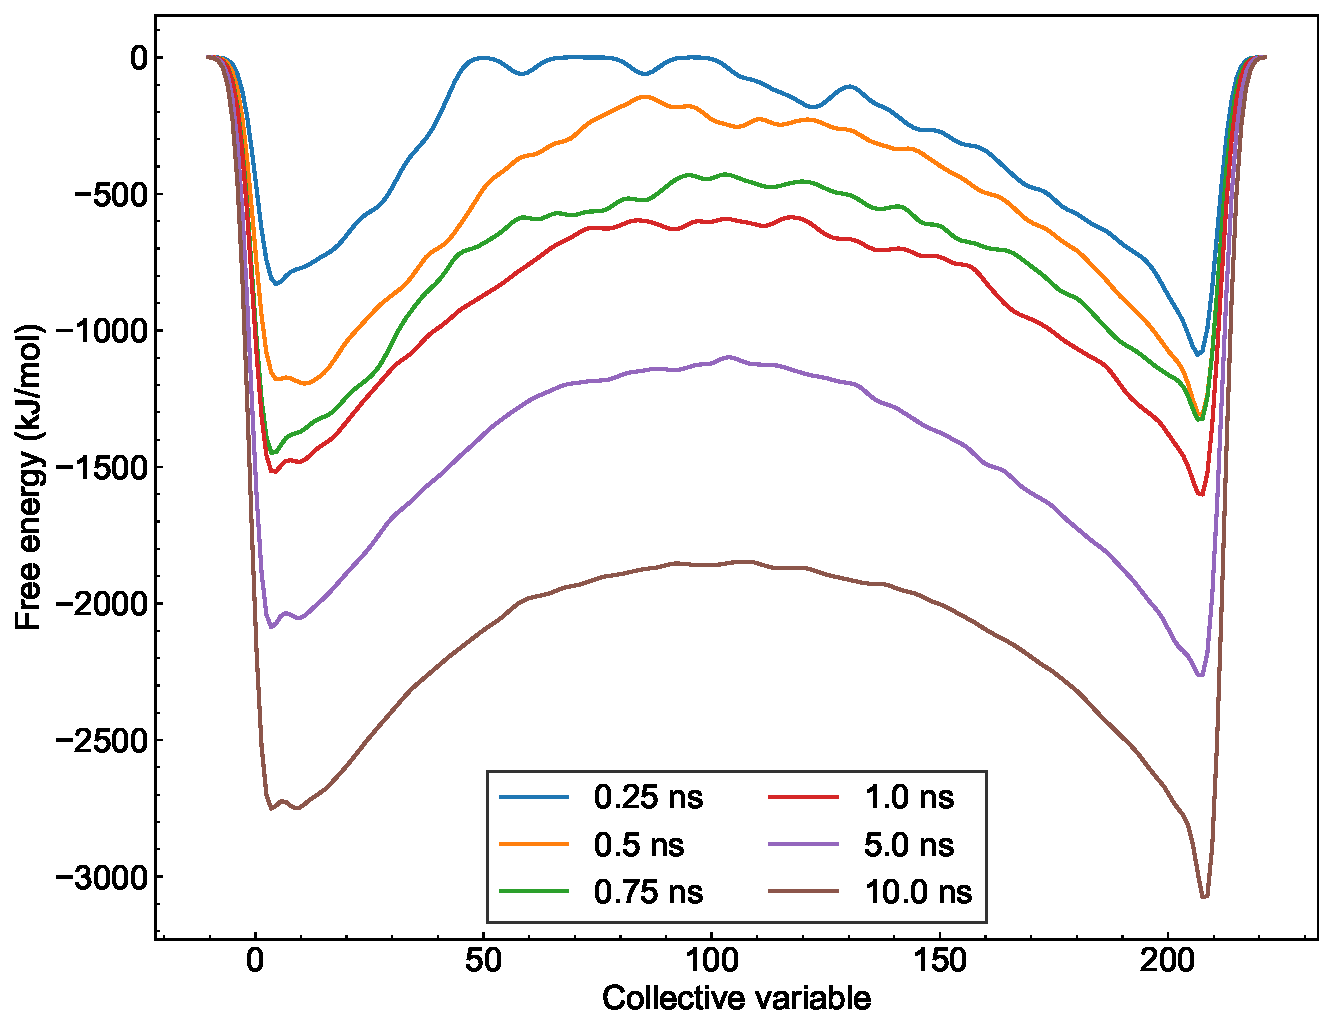
\includegraphics[width=0.8\textwidth]{./plot/conv.pdf}
    \caption{The convergence of the free energy surface of silicon as a function of simulation time at 1700 K.}
\end{figure}

\begin{figure}[p]
    \centering
    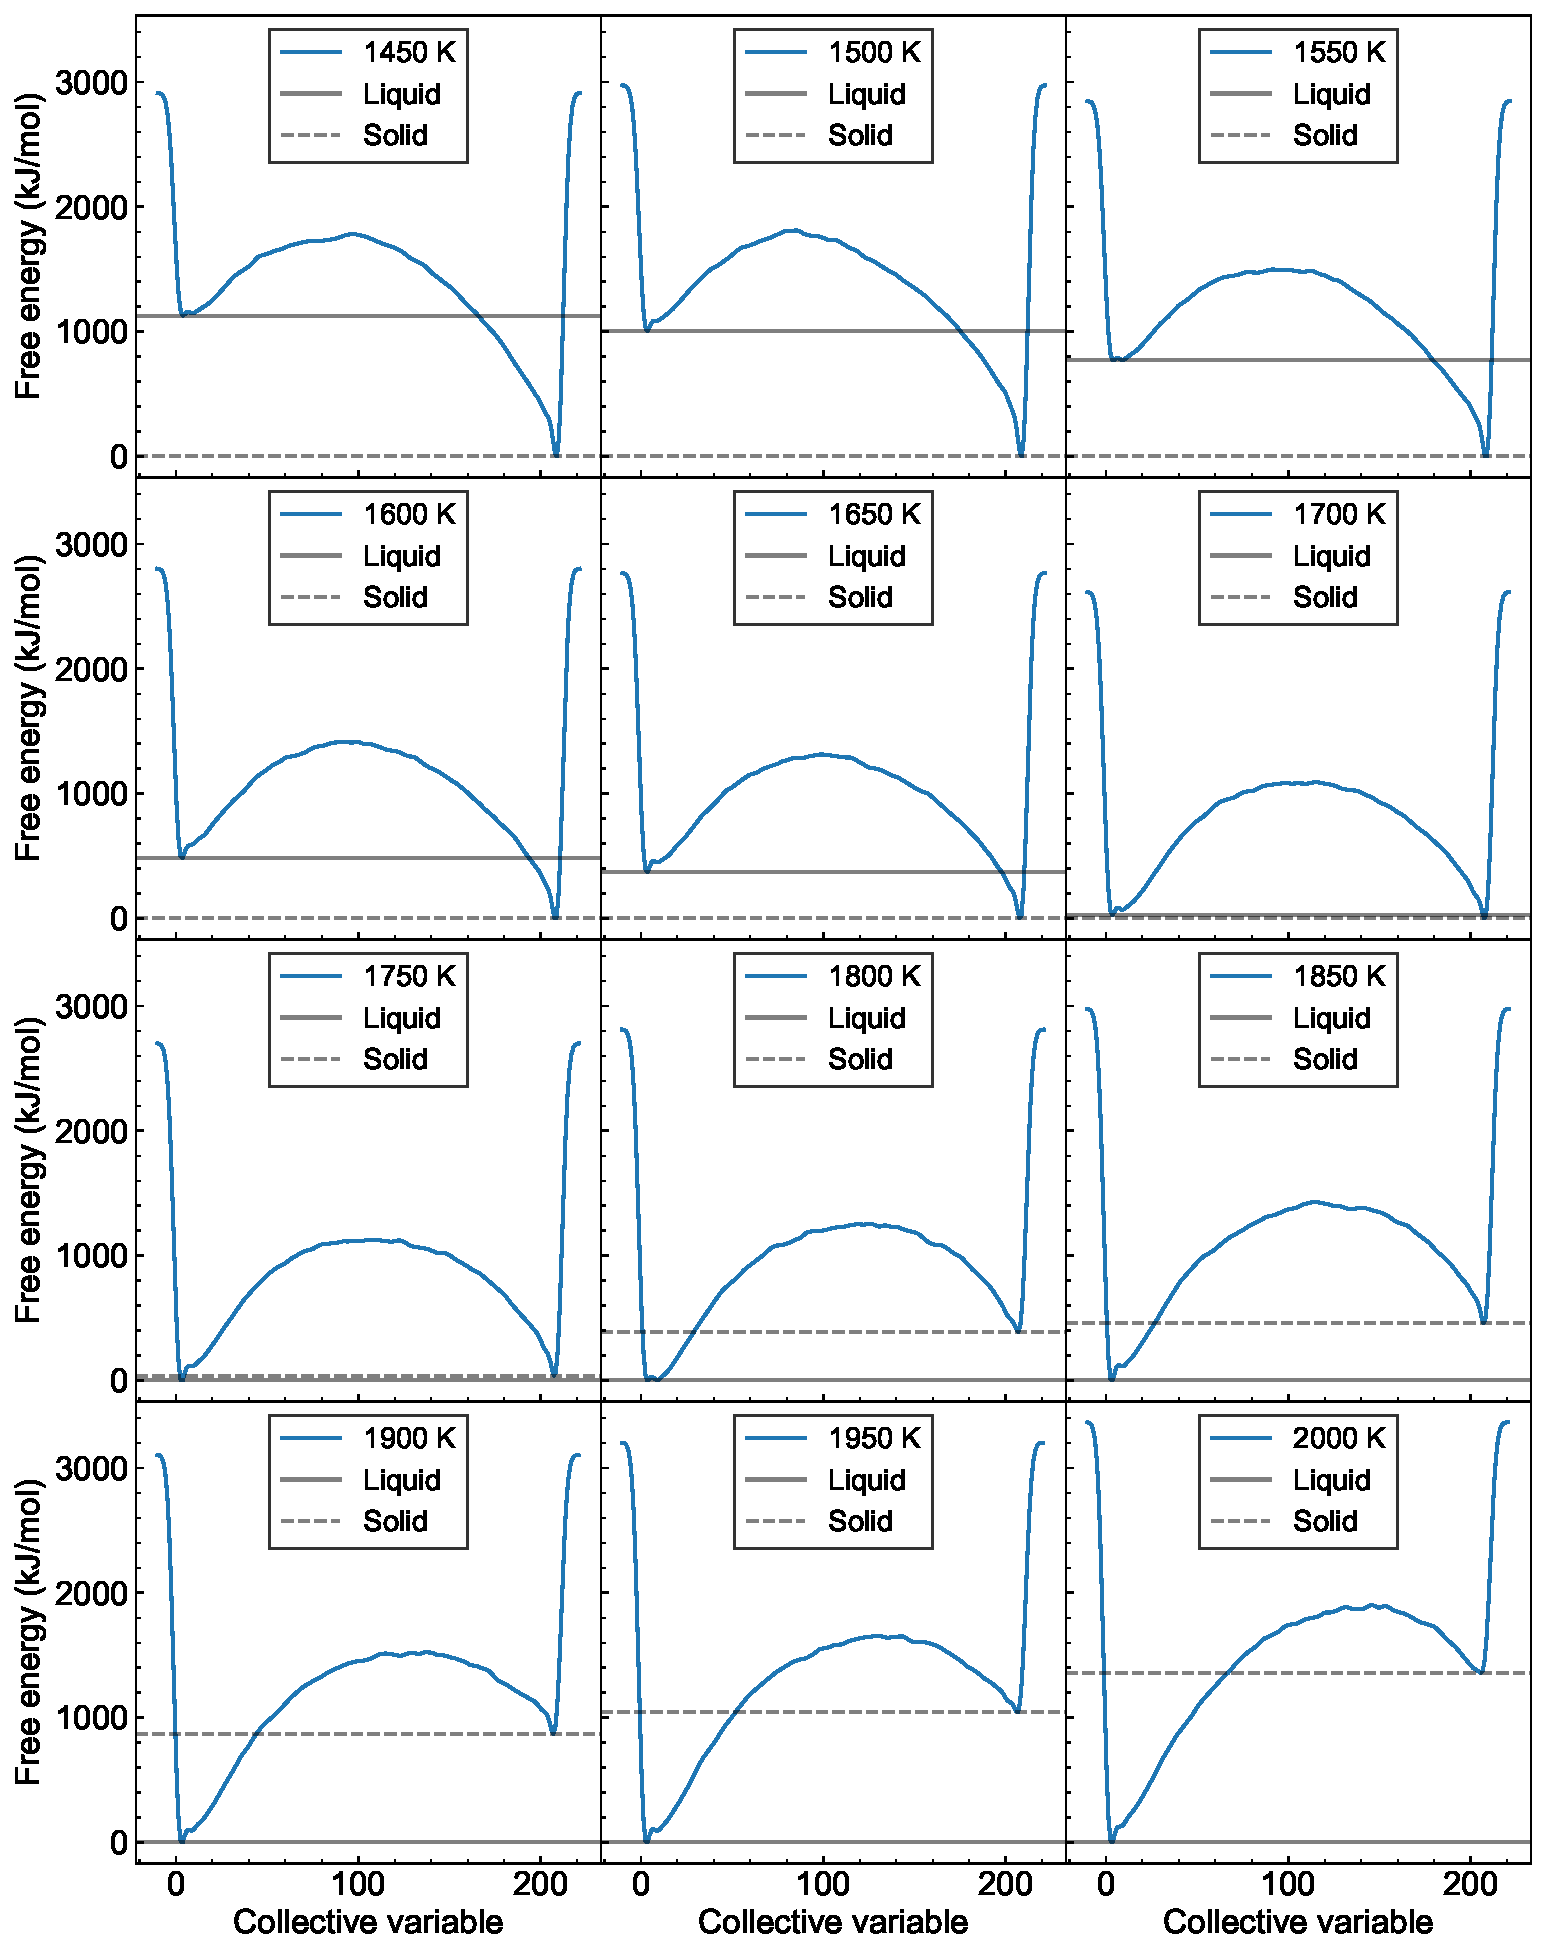
\includegraphics[width=\textwidth]{./plot/fes.pdf}
    \caption{The free energy surface of silicon at different temperatures for a 216-atom system.}
\end{figure}

In the simulation, I obtain a free energy profile at each temperature spanning liquid and solid basins and the barrier in between. I take a 216-atom system at 1700 K as an example to study the convergence of the free energy surface (FES). 

The FES is calculated by the command \verb|$plumedexe sum_hills --hills HILLS --stride=250|, which gives the FES as a function of simulation time every 250 ps. The results are shown in Fig. 1. It suggests that during the first ns the shape of the FES changes substantially. After this simulation time the overarching structure of the FES remains relatively stable, with only minor features being refined. Best on the results, a 10-ns trajectory is enough for the convergence of the FES and for the study of the crystallization of silicon.

\subsection{The free energy surface at different temperatures}

The FES at different temperatures are plotted and shown in Fig. 2. At 1700 K and 1750 K, the two free energy minima, i.e., the liquid basin on the left and the solid basin on the right, are at approximately the same free energy, which means that they are close to the coexistence temperature. As the temperature varies from the coexistence value one or the other of the two basins becomes deeper, corresponding to an undercooled liquid or an overheated crystal. Therefore, the melting temperature of silicon is between 1700 K and 1750 K based on my simulations of a 216-atom system.

\subsection{The liquid-solid free energy difference and the melting temperature}

The difference in free energy between the liquid and the solid can be approximated as a difference in height between the two free energy minima. In order to more accurately determine the melting temperature, I calculated the free energy difference between the liquid phase and solid phase at different temperatures and I found that the difference in free energy has a very good linear relationship with temperature when it is close to the melting temperature. Therefore, I used the least squares method to perform a linear fit for the liquid-solid free energy difference versus temperature, and determined the melting temperature by identifying the intercept of the fitted line on the x-axis, as shown in Fig. 3. The results show that the melting temperature of silicon obtained by metadynamics simulations with 216 atoms is $1720 \pm 74$ K, where the error bar is somewhat overestimated which is calculated through the error propagation rule based on the root-mean-square of the residuals from the linear fit (the standard deviation of the linear fit).

\begin{figure}[t]
    \centering
    \subfloat[216 atoms]
    {
    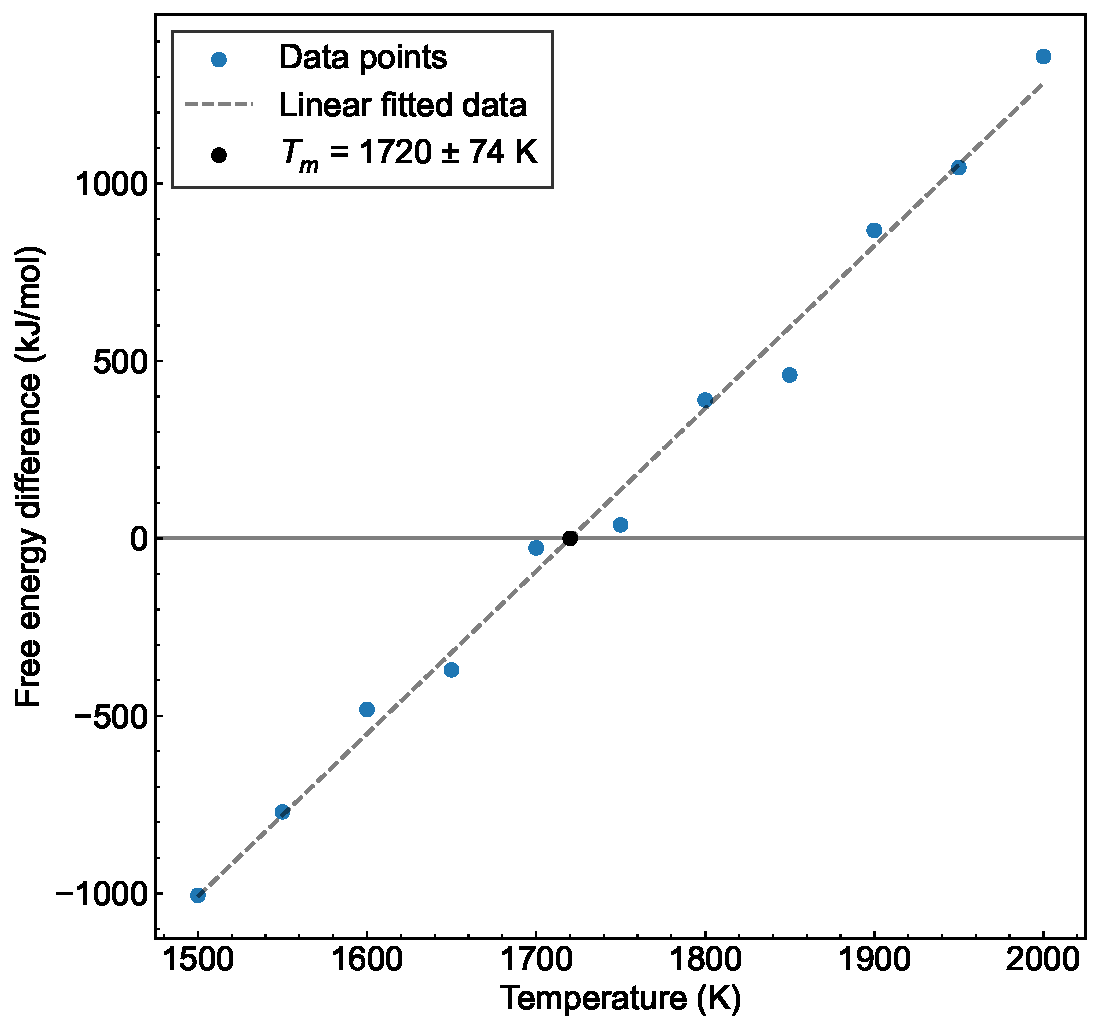
\includegraphics[width=0.5\textwidth]{plot/diff-333.pdf}
    }
    \subfloat[1000 atoms]
    {
    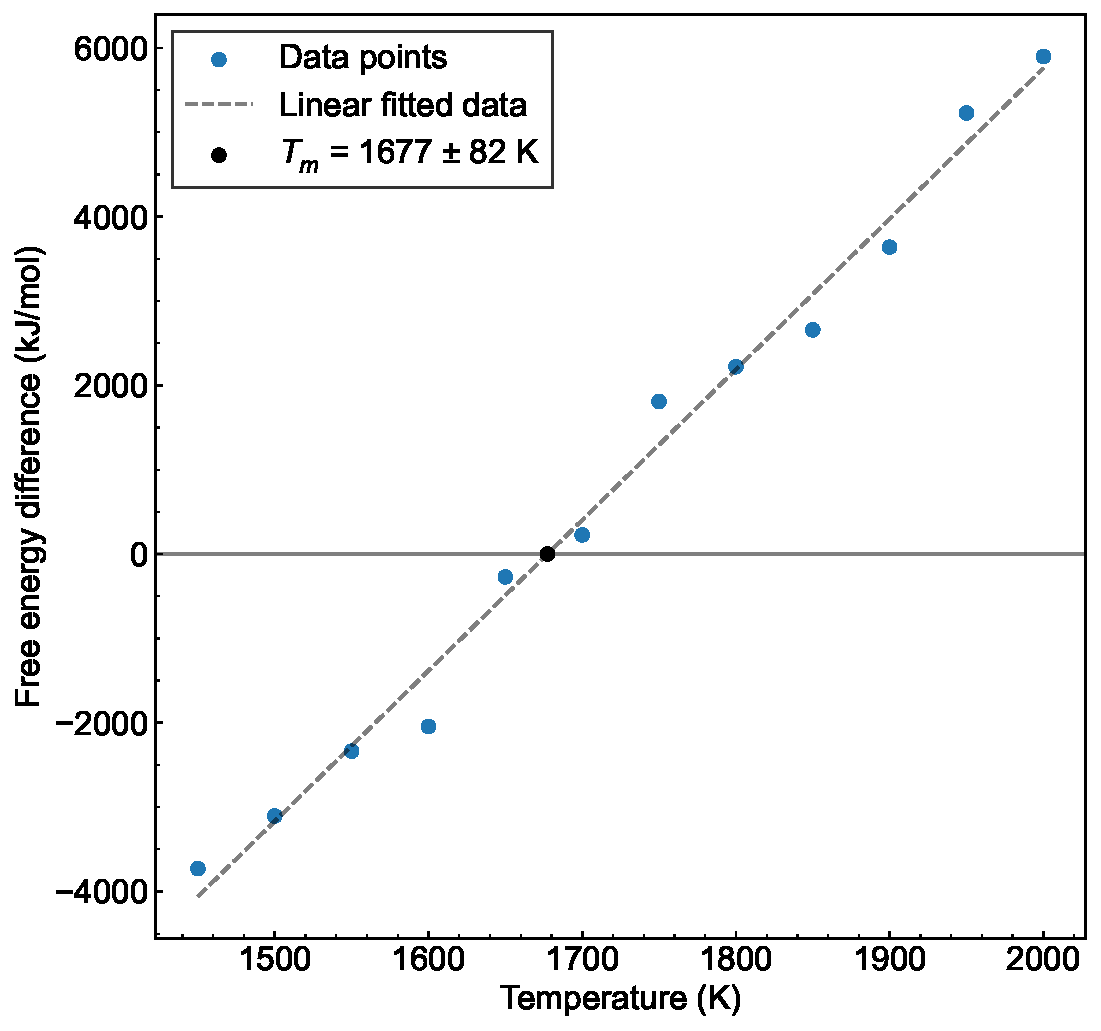
\includegraphics[width=0.5\textwidth]{plot/diff-555.pdf}
    }
    \caption{The difference in free energy between the liquid and the solid as a function of temperature. The plot for the 216-atom system and the 1000-atom system are shown as examples.}
\end{figure}

\begin{figure}[h!]
    \centering
    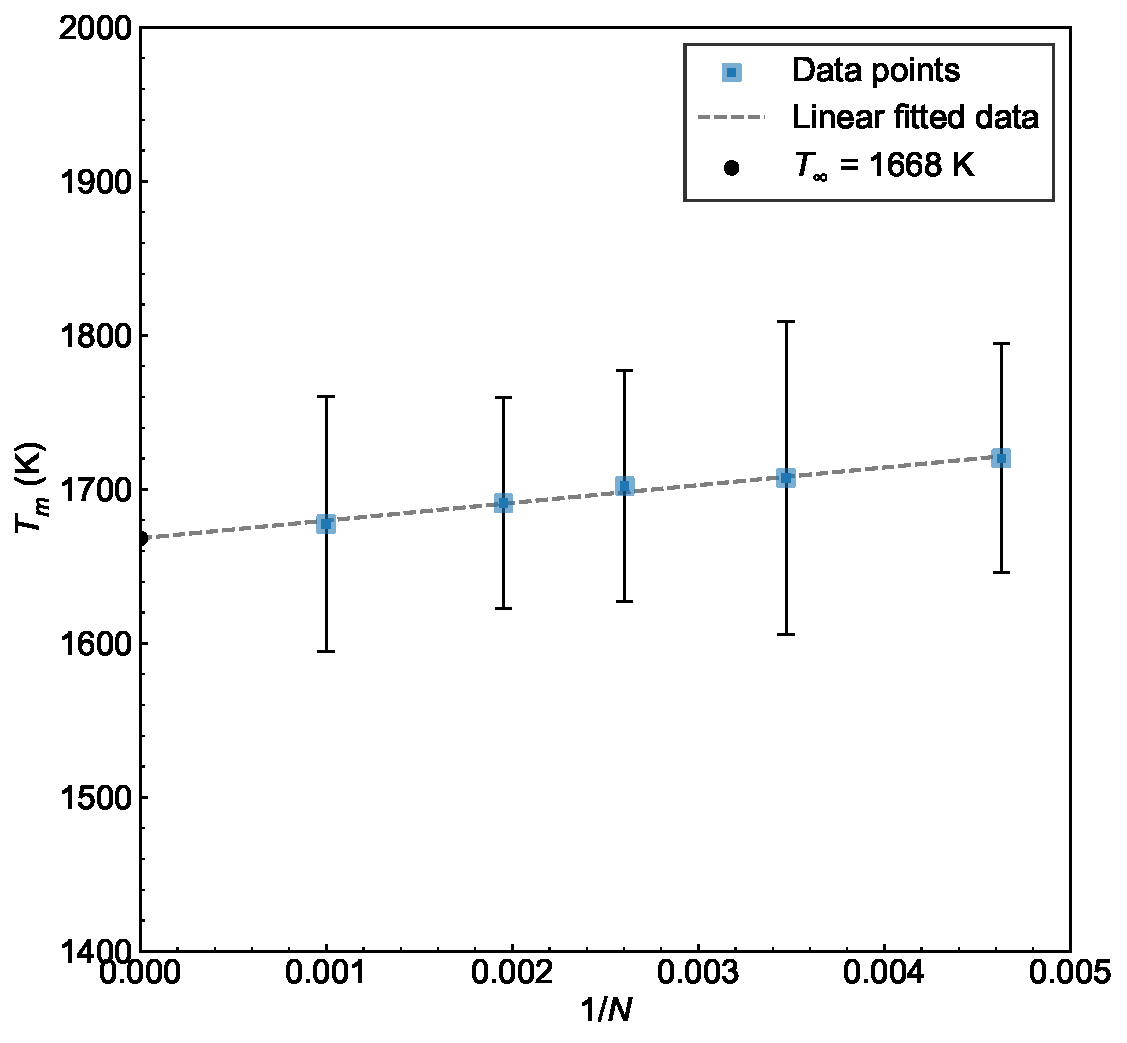
\includegraphics[width=0.7\textwidth]{./plot/size.pdf}
    \caption{The size effect of the melting temperature.}
\end{figure}

\subsection{The size effect of the melting temperature}

When considering finite size systems, like the systems in this project, the behavior at the phase transition changes slightly. Due to the finite number of particles, the sharp discontinuity seen in infinite systems gets smoothed out. Moreover, fluctuations become more important as the size of the system decreases. Using the method described in Section 3.3, I calculate the melting temperatures of silicon for systems with different sizes (Table. 1), and plot the melting temperature as a function of reciprocal atom numbers, as shown in Fig. 4. Finite size scaling theory for first order phase transitions predicts a linear relationship between the melting temperature and the inverse of the number of particles. Therefore, the size effect for $T_m$ is given by
\begin{equation}
    T_m(N) = T_{\infty} + \frac{A}{N}
\end{equation}
where $T_{\infty}$ is the thermodynamic limit of $T_m$ with infinite size, $N$ is the number of particles, and $A$ is a constant. By fitting this extrapolation formula to the $T_m$ results, I find that the melting temperature at the thermodynamic limit is $T_{\infty} = 1668$ K.

\subsection{Determine the optimal SIGMA parameter}
One of the parameters that has to be chosen is SIGMA in the definition of the collective variable. One way to choose an appropriate SIGMA is by analyzing the distributions of kernel
\begin{equation}
    k_{\chi_0}(\chi)=\int d \mathbf{r} \rho_\chi(\mathbf{r}) \rho_{\chi_0}(\mathbf{r})
\end{equation}
in the liquid and the solid, where $\rho_\chi(\mathbf{r})$ is the atomic density around environment $\chi$. We can then determine the overlap between these distributions and choose the value of SIGMA that minimizes the overlap, therefore maximizing the ability of the CV to discriminate between structures. 

I run MD simulations without enhanced sampling of the liquid and the solid at 1720 K. For the liquid phase, I first perform an NPT simulation at 2500 K to melt the silicon with diamond lattice, and then equilibrate the system to 1720 K. I then postprocess these simulations using PLUMED and calculate the distributions of the kernel for different values of SIGMA, as shown in Fig. 6. We can measure the overlap between the distributions using
\begin{equation}
    \textrm{Overlap} = \int dx \min[ P_1(x), P_2(x) ] 
\end{equation}
The overlap as a function of SIGMA is calculated and shown in Fig 5. This gives an optimum value of SIGMA of $\sim$0.067 nm. In the case of silicon the overlap between distributions is very small for most values of SIGMA because the structure of the liquid and the solid are very different, so I have used SIGMA = 0.04 nm. This is not the case for every substance and choosing SIGMA carefully can help to discriminate better between phases. 

\begin{figure}[h!]
    \centering
    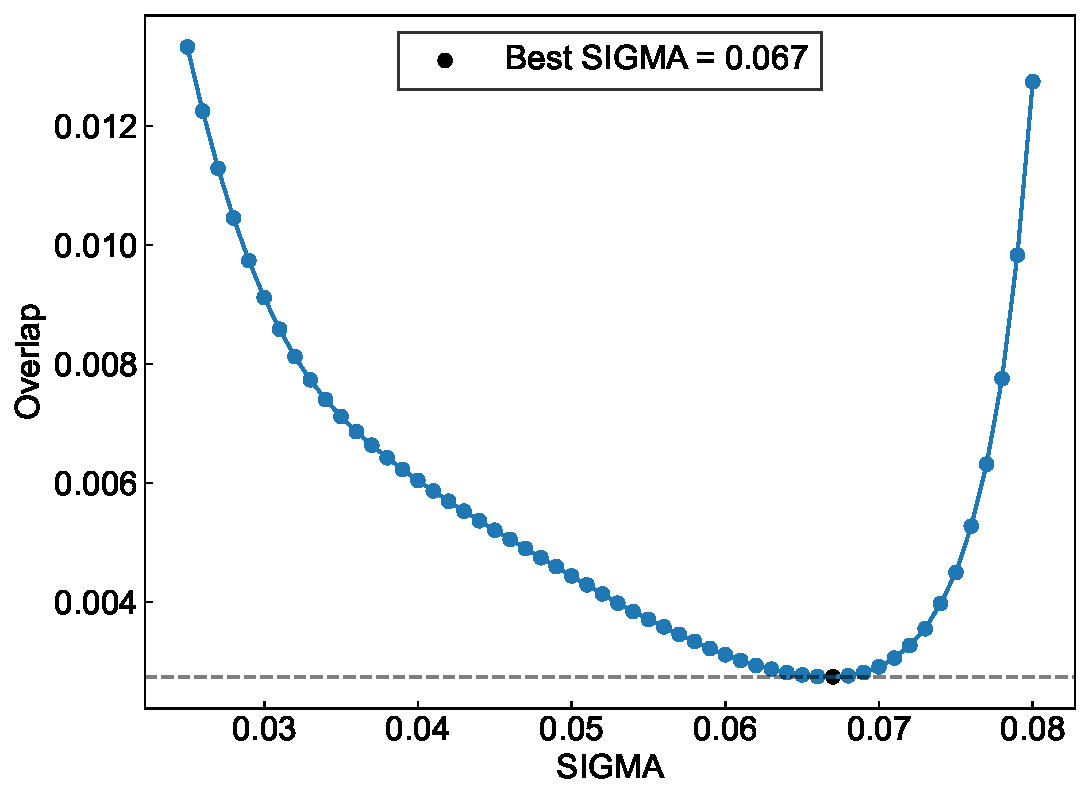
\includegraphics[width=0.85\textwidth]{./plot/overlap.pdf}
    \caption{The overlap between the distributions for different values of SIGMA at 1720 K.}
\end{figure}

\begin{figure}[p]
    \centering
    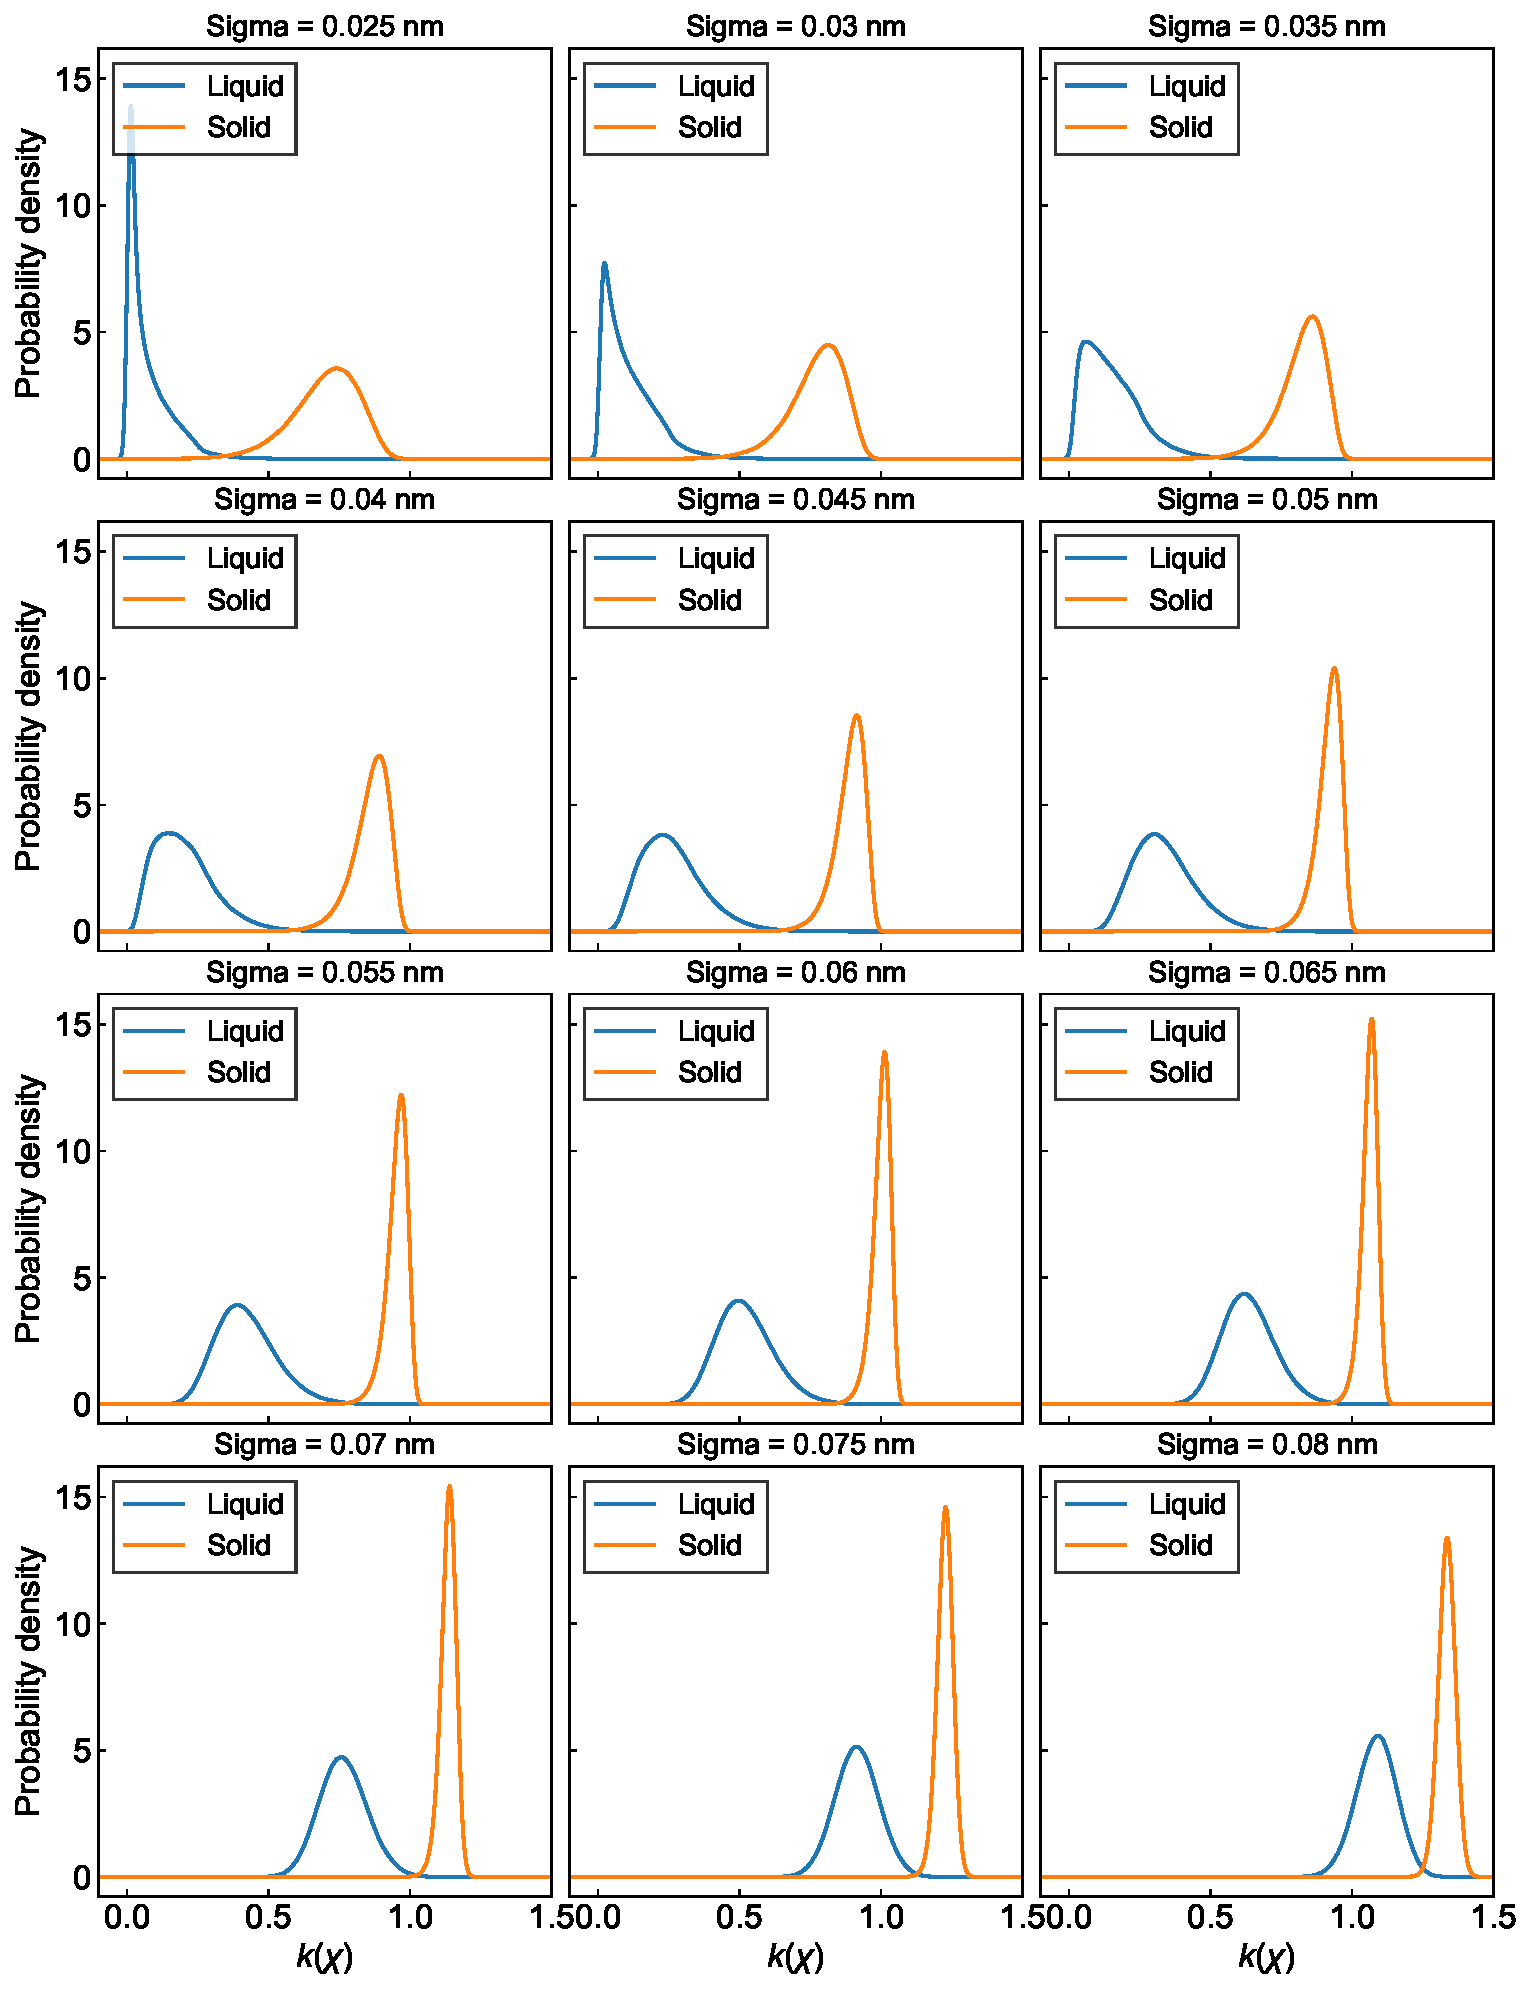
\includegraphics[width=\textwidth]{./plot/histo.pdf}
    \caption{The distributions of the kernel $\rho_\chi(\mathbf{r})$ for different values of SIGMA at 1720 K.}
\end{figure}

\subsection{Calculate the thermodynamic properties}

\begin{figure}[h!]
    \centering
    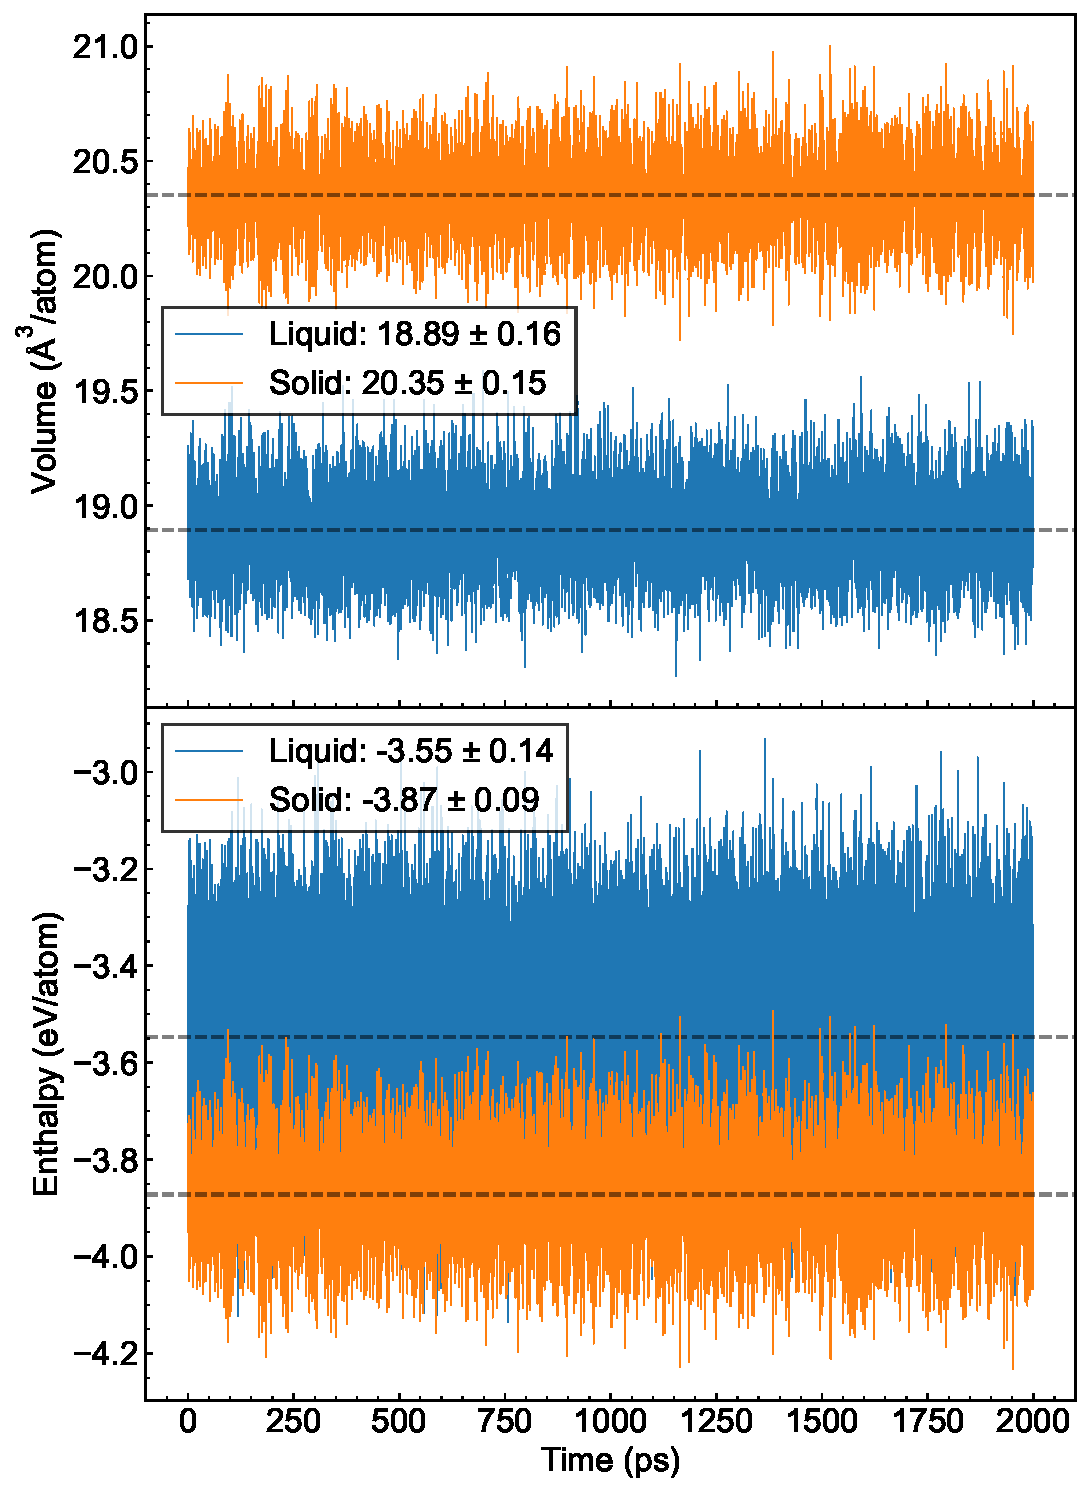
\includegraphics[width=0.7\textwidth]{./plot/props.pdf}
    \caption{The specific volume and specific enthalpy of solid and liquid silicon as a function of simulation time at 1720 K.}
\end{figure}

From the simulations I can also estimate some thermodynamic properties of silicon, including the latent heat of fusion which is the enthalpy change from solid to liquid, the specific volumes of the solid and the liquid, and the volume discontinuity at melting. To achieve this, I run MD simulations without enhanced sampling of the liquid and the solid at 1720 K, which is the melting temperature of the 216-atom system. For the liquid phase, I first perform an NPT simulation at 2500 K to melt the silicon with diamond lattice, and then equilibrate the system to 1720 K. The total simulation time is 2 ns with a time step of 2 fs. I use the \verb|thermo_style| command in LAMMPS input file to output the volume and enthalpy of the system. The fluctuation of specific volume and specific enthalpy for both solid and liquid silicon are shown in Fig. 7. My results for latent heat ($\Delta H_{sl}$), specific volumes ($V_s$ and $V_l$), and volume discontinuity at melting ($\Delta V$) are shown in Table 2, as well as corresponding experimental values. It's worth noting that the unit of specific volume in the experimental values is a.u.$^3$, while the output of LAMMPS is in \AA$^3$, so I need to convert the unit for my results. Overall, my simulation results agree well with the experiment, but the calculated latent heat and volume discontinuity are relatively lower than the experimental values.

\begin{table}[h!]
    \centering
    \caption{Thermodynamic properties of silicon obtained from MD simulations and experiments. The error is the standard deviation throughout the MD trajectory.}
    \begin{tabular}{ccc}
    \toprule
                                & This work        & Experiment \\ \midrule
    $T_m$ (K)                   & 1668             & 1685       \\
    $\Delta H_{sl}$ (eV/atom)   & $0.33 \pm 0.16$  & 0.52; 0.47 \\
    $V_s$ (a.u.$^3$/atom)       & $137.3 \pm 1.0$  & 138.0      \\
    $V_l$ (a.u.$^3$/atom)       & $127.5 \pm 1.1$  &            \\
    $\Delta V$ (a.u.$^3$/atom)  & $9.83 \pm 1.45$  &            \\
    $\Delta V/V_s$ (\%)         & $7.16 \pm 1.02$  & 11.9; 9.5  \\ \bottomrule
    \end{tabular}
\end{table}

\section{Limitations}

The computer simulation of melting processes using enhanced sampling methods is a powerful tool for understanding these processes at a molecular level. However, it's important to point out that these simulations are indeed simplified models of reality. Here are some possible reasons:
\begin{enumerate}
    \item Nucleation: Nucleation is the realistic process during the formation of new phases. It begins with the formation of small clusters, which can grow if they are thermodynamically stable. The process of nucleation is stochastic and depends on fluctuations, which might not be well captured in a computer simulation, particularly if the system size is small. Moreover, classical nucleation theory, which is often used to understand these processes, makes certain simplifying assumptions (e.g., that the new phase is a perfect sphere) that may not hold in reality.
    \item Model limitations: The Stillinger-Weber (SW) potential is an empirical potential, meaning that it's based on fitting experimental data rather than first principles. It may not correctly describe some properties of silicon outside those data, and may not account for certain types of defects or surface effects.
    \item Metadynamics: While metadynamics is a powerful enhanced sampling method, it's also based on certain approximations. For example, the choice of collective variables and the form of the bias potential can greatly influence the results. Moreover, metadynamics samples the free energy surface by adding a history-dependent bias potential, which is an approximation to the true dynamics of the system.
    \item Quantum effects: In real physical systems, especially at low temperatures or for light atoms, quantum effects can become important. Classical molecular dynamics simulations, like those using the Stillinger-Weber potential, don't capture these quantum effects.
    \item Thermodynamic conditions: Simulations are typically performed under specific thermodynamic conditions (e.g., constant temperature or pressure), which may not perfectly match real-world conditions. In reality, conditions may vary locally and with time, leading to a more complex behavior.
\end{enumerate}
In conclusion, while computer simulations are useful tools for understanding complex physical processes like crystallization and melting, it's important to keep in mind their limitations and the approximations involved.

\end{document}
